\documentclass[journal,12pt,twocolumn]{IEEEtran}

\usepackage{setspace}
\usepackage{gensymb}
\singlespacing
\usepackage[cmex10]{amsmath}
\usepackage{amsmath}

\usepackage{amsthm}

\usepackage{mathrsfs}
\usepackage{txfonts}
\usepackage{stfloats}
\usepackage{bm}
\usepackage{cite}
\usepackage{cases}
\usepackage{subfig}

\usepackage{longtable}
\usepackage{multirow}
\usepackage{caption}

\usepackage{enumitem}
\usepackage{mathtools}
\usepackage{steinmetz}
\usepackage{tikz}
\usepackage{circuitikz}
\usepackage{verbatim}
\usepackage{tfrupee}
\usepackage[breaklinks=true]{hyperref}
\usepackage{graphicx}
\usepackage{tkz-euclide}
\usepackage{float}
\usepackage{mathtools}

\usetikzlibrary{calc,math}
\usepackage{listings}
    \usepackage{color}                                            %%
    \usepackage{array}                                            %%
    \usepackage{longtable}                                        %%
    \usepackage{calc}                                             %%
    \usepackage{multirow}                                         %%
    \usepackage{hhline}                                           %%
    \usepackage{ifthen}                                           %%
    \usepackage{lscape}     
\usepackage{multicol}
\usepackage{chngcntr}

\DeclareMathOperator*{\Res}{Res}
\newcommand*{\permcomb}[4][0mu]{{{}^{#3}\mkern#1#2_{#4}}}
\newcommand*{\perm}[1][-3mu]{\permcomb[#1]{P}}
\newcommand*{\comb}[1][-1mu]{\permcomb[#1]{C}}
\renewcommand\thesection{\arabic{section}}
\renewcommand\thesubsection{\thesection.\arabic{subsection}}
\renewcommand\thesubsubsection{\thesubsection.\arabic{subsubsection}}

\renewcommand\thesectiondis{\arabic{section}}
\renewcommand\thesubsectiondis{\thesectiondis.\arabic{subsection}}
\renewcommand\thesubsubsectiondis{\thesubsectiondis.\arabic{subsubsection}}


\hyphenation{op-tical net-works semi-conduc-tor}
\def\inputGnumericTable{}                                 %%

\lstset{
%language=C,
frame=single, 
breaklines=true,
columns=fullflexible
}
\begin{document}

\newcommand{\BEQA}{\begin{eqnarray}}
\newcommand{\EEQA}{\end{eqnarray}}
\newcommand{\define}{\stackrel{\triangle}{=}}
\bibliographystyle{IEEEtran}
\raggedbottom
\setlength{\parindent}{0pt}
\providecommand{\mbf}{\mathbf}
\providecommand{\pr}[1]{\ensuremath{\Pr\left(#1\right)}}
\providecommand{\qfunc}[1]{\ensuremath{Q\left(#1\right)}}
\providecommand{\sbrak}[1]{\ensuremath{{}\left[#1\right]}}
\providecommand{\lsbrak}[1]{\ensuremath{{}\left[#1\right.}}
\providecommand{\rsbrak}[1]{\ensuremath{{}\left.#1\right]}}
\providecommand{\brak}[1]{\ensuremath{\left(#1\right)}}
\providecommand{\lbrak}[1]{\ensuremath{\left(#1\right.}}
\providecommand{\rbrak}[1]{\ensuremath{\left.#1\right)}}
\providecommand{\cbrak}[1]{\ensuremath{\left\{#1\right\}}}
\providecommand{\lcbrak}[1]{\ensuremath{\left\{#1\right.}}
\providecommand{\rcbrak}[1]{\ensuremath{\left.#1\right\}}}
\theoremstyle{remark}
\newtheorem{rem}{Remark}
\newcommand{\sgn}{\mathop{\mathrm{sgn}}}
\providecommand{\abs}[1]{\vert#1\vert}
\providecommand{\res}[1]{\Res\displaylimits_{#1}} 
\providecommand{\norm}[1]{\lVert#1\rVert}
%\providecommand{\norm}[1]{\lVert#1\rVert}
\providecommand{\mtx}[1]{\mathbf{#1}}
\providecommand{\mean}[1]{E[ #1 ]}
\providecommand{\fourier}{\overset{\mathcal{F}}{ \rightleftharpoons}}
%\providecommand{\hilbert}{\overset{\mathcal{H}}{ \rightleftharpoons}}
\providecommand{\system}{\overset{\mathcal{H}}{ \longleftrightarrow}}
	%\newcommand{\solution}[2]{\textbf{Solution:}{#1}}
\newcommand{\solution}{\noindent \textbf{Solution: }}
\newcommand{\cosec}{\,\text{cosec}\,}
\providecommand{\dec}[2]{\ensuremath{\overset{#1}{\underset{#2}{\gtrless}}}}
\newcommand{\myvec}[1]{\ensuremath{\begin{pmatrix}#1\end{pmatrix}}}
\newcommand{\mydet}[1]{\ensuremath{\begin{vmatrix}#1\end{vmatrix}}}
\numberwithin{equation}{subsection}
\makeatletter
\@addtoreset{figure}{problem}
\makeatother
\let\StandardTheFigure\thefigure
\let\vec\mathbf
\renewcommand{\thefigure}{\theproblem}
\def\putbox#1#2#3{\makebox[0in][l]{\makebox[#1][l]{}\raisebox{\baselineskip}[0in][0in]{\raisebox{#2}[0in][0in]{#3}}}}
     \def\rightbox#1{\makebox[0in][r]{#1}}
     \def\centbox#1{\makebox[0in]{#1}}
     \def\topbox#1{\raisebox{-\baselineskip}[0in][0in]{#1}}
     \def\midbox#1{\raisebox{-0.5\baselineskip}[0in][0in]{#1}}
\vspace{3cm}
\title{Assignment-2}
\author{Name: Sai Pravallika Danda, Roll Number: CS20BTECH11013}
\maketitle
\newpage
\bigskip
\renewcommand{\thefigure}{\theenumi}
\renewcommand{\thetable}{\theenumi}
Download all python codes from 
\begin{lstlisting}
https://github.com/spdanda/AI1103/tree/main/Assignment2/codes
\end{lstlisting}
%
and latex-tikz codes from 
%
\begin{lstlisting}
https://github.com/spdanda/AI1103/blob/main/Assignment2/Assignment2.tex
\end{lstlisting}
\large\textbf{Problem 5.31 :}\\
Two cards are drawn simultaneously (or successively without replacement) from a well-shuffled  pack  of  52  cards.  Find  the  mean, variance and standard deviation of the number of kings.\\
\textbf{Solution :}\\
Let X denote the no.of kings in a draw of 2 cards.
\begin{align}
\implies \Pr(\emph{X}=0) &= \dfrac{\comb{48}{2}}{\comb{52}{2}}=\dfrac{188}{221} \\
\Pr(\emph{X}=1) &= \dfrac{{\comb{4}{1}} \times {\comb{48}{1}}}{{\comb{52}{2}}}=\dfrac{32}{221} \\ 
\Pr(\emph{X}=2)&=\dfrac{\comb{4}{2}}{\comb{52}{2}}= \dfrac{1}{221}\\ \nonumber
\end{align}

\begin{center}
\begin{table}[h]
    \centering
    \resizebox{\columnwidth}{!}{
\begin{tabular}{|c|c|c|}
\hline
SNo. & Case & Probability of the case \\
\hline
1 & $\Pr(X=0)$ & 188/221 \\ 
\hline
2 & $\Pr(X=1)$ & 32/221 \\ 
\hline
3 & $\Pr(X=2)$ & 1/221 \\
\hline
\end{tabular}
}
    \caption{\large Probability distribution table }
    \label{table 1}
\end{table}
\end{center}

\newpage

\begin{align}
 \text{Mean of \emph{X}}&= \emph{E(X)} \\  
               &=\sum_{\emph{k}=0}^{2}   k\Pr(\emph{X=k})\\ 
               &=1 \times\frac{32}{221}+2 \times\frac{1}{221}\\
               &= \frac{34}{221} = 0.154\\ \nonumber
\end{align}

\begin{align}
 \text{Variance} &=\emph{E}(\emph{X}^2) - [\emph{E}(\emph{X})]^2\\ 
                  &= \sum_{\emph{k}=0}^{2} \emph{k}^2 \Pr(\emph{X=k}) - \frac{34^2}{221^2}\\ 
                  &= 1^2\times\frac{32}{221} + 2^2\times\frac{1}{221} - \frac{34^2}{221^2}\\\vspace{0.1cm}
                  &= \frac{6800}{48841} = 0.139\\ \nonumber
\end{align}

\begin{align}
 \text{Standard Deviation }\sigma &= \sqrt{\emph{Var(X)}}\\  
&= \sqrt{0.139}\\ &= 0.373\\ \nonumber
\end{align}

\newpage
\begin{figure}[h!]
    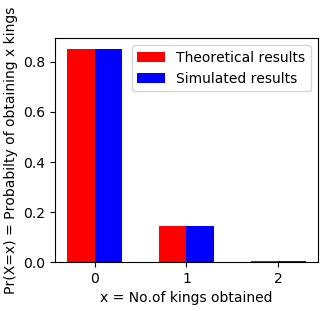
\includegraphics{Fig1.png}
    \caption{\large Theoretical and Simulated probability results}
\end{figure}


\end{document}